\chapter{\medullotitle}
\label{chap:medullo}
\glsresetall
\clearpage

\section{Abstract}
\par\textit{Motivation ---} \Gls{MB} is the most common malignant pediatric brain tumor. The current standard of care for \gls{MB} consists of maximal safe resection followed by chemotherapy and/or radiation, and carries substantial risk of co-morbidity and secondary neoplasms. So far, targeted molecular therapies have failed to reliably achieve sustained remission. Notably, the genomic features of \gls{MB} subgroups with the worst prognoses, namely \textit{TP53} inactivation and \textit{MYC} family amplification, are also associated with ecDNA in other tumor types. We therefore asked whether \gls{ecDNA} may be a prognostic biomarker of patient survival in \gls{MB}, and investigated the genomes of \gls{ecDNA} sequences found in \gls{MB} patient tumors to elucidate their possible oncogenic roles.
\par\textit{Results ---} In \gls{MB}, the presence of ecDNA in a tumor sample correlates with other known molecular prognostic indicators, namely \textit{TP53} mutation and \textit{MYC} gene family amplification, and is itself strongly associated with poor progression-free survival. We propose a causal model whereby \textit{TP53} inactivation promotes genome instability, which may affect response to therapy by the formation of ecDNA or by the formation of other structural variants.
\par\textit{Availability and implementation ---} This chapter summarizes work from the following publication: \cite{Chapman}
Code is available at \url{https://github.com/auberginekenobi/medullo-ecdna}.  

\section{Introduction}
\par Circular extrachromosomal DNA (ecDNA), defined as circular, acentric megabase-scale genomic DNA found exclusively in cancer cells \cite{Verhaak_2019, bafna_2022}, has been associated with high-copy oncogenic amplification \cite{Turner_2017}, intratumoral heterogeneity \cite{Lange_2021, xu_2019}, evolution of targeted therapy resistance \cite{decarvalho_2018,Nathanson_2014}, and poor patient outcomes across various tumor types \cite{Kim_2020, Koche_2020}. Although the frequency, sequence content, and prognostic value of ecDNA is well-described in various adult solid tumor types \cite{Kim_2020} and pediatric neuroblastoma \cite{Koche_2020}, the clinical presentation of ecDNA in \gls{MB} has not yet been described. Therefore, there is compelling need to survey the frequency, genomic sequence, and prognostic utility of ecDNA across the molecular subgroups of \gls{MB}, to determine how extrachromosomal amplification may affect the response of a tumor to the current standards of care. Here we computationally screen for ecDNA across a large cohort of \gls{wgs} of pediatric solid tumors from the St. Jude Cloud \cite{stjude}, \gls{icgc}, and \gls{cbtn} \cite{cbtn}, and identify key clinical and genomic features of ecDNA in \gls{MB}.

\par Medulloblastomas were represented among the first patient case reports describing ecDNA \cite{Cox_1966,Herbert_1965}, and several patient-derived cell line models of MB are known to contain ecDNA \cite{Morton_2019}. Few effective targeted molecular treatments exist for MB, and the current standard of care carries substantial risk of developmental disorder, neurological damage, and secondary metastasis \cite{Salloum_2019}. There are four major molecular subgroups of MB: WNT, SHH, Group 3 (G3) and Group 4 (G4) \cite{Juraschka_2019}. Prognosis is especially poor for a subset of aggressive MYC-activated Group 3 tumors, and for p53-mutant SHH subgroup tumors \cite{Northcott_2017,Ramaswamy_2016}. Both \textit{MYC} amplification and p53 mutation have been co-reported alongside ecDNA in MB \cite{Ryan_2012,Rausch_2012}, but the strength of any possible association has not yet been quantified in a patient population. Although the genomic landscape of medulloblastoma subgroups has been largely characterized \cite{Northcott_2017}, it remains unknown how frequently ecDNA occurs in MB patients, and whether the presence of ecDNA may affect prognosis or correlate with other molecular features. 

\section{Results}

\subsection{ecDNA amplifies known and putative medulloblastoma oncogenes.}
To examine the landscape of ecDNA in medulloblastoma, we accessed \acrshort{wgs} data available in three cancer cloud genomics platforms: St Jude Cloud \cite{stjude}, the \acrfull{cbtn} \cite{cbtn}, and the \acrfull{icgc} \cite{pcawg}. In addition, we included 43 tumors from a previous proteomic analysis \cite{archer_2017} and 8 tumors from MB patients diagnosed at the Rady Children's Hospital, San Diego. In total, we analyzed a retrospective cohort of WGS data of 481 tumor biopsies from 468 different patients. Using DNA fingerprint analysis, we ensured that the combined cohort WGS data contained no duplicate specimens (see section \ref{chap1:methods}). Clinical metadata were available for most patients and included age at diagnosis, sex, MB molecular subgroup, and survival (Suppl. Tbl. 1 from \cite{Chapman}). To detect ecDNA, we applied AmpliconArchitect (AA), an algorithm that detects ecDNA using paired-end WGS data \cite{AA}. 102 putative ecDNA sequences were detected in tumor samples from 82 of 468 (18\%) patients. By molecular subgroup, ecDNA+ patients were distributed as follows: WNT 0/22, SHH 30/112 (27\%), Group 3 19/107 (18\%), and Group 4 26/181 (14\%) (Fig. \ref{fig:1a}). SHH subgroup tumors were significantly more likely to contain ecDNA than tumors from the other MB subgroups ($\chi^2=7.66$, $p=0.006$). Among the ecDNA-amplified genes occurring in two or more samples in this cohort were known or suspected MB oncogenes \textit{MYC}, \textit{MYCN}, \textit{MYCL1}, \textit{TERT}, \textit{GLI2}, \textit{CCND2} (Cyclin D2) \cite{garancher_2018}, \textit{PPM1D} (WIP1) \cite{Wen_2016}, and \textit{ACVR2B} \cite{morabito_2019}; members of signaling pathways commonly dysregulated in cancer, such as DNA repair (\textit{RAD51AP1} and \textit{RAD21}); and p53 pathway inhibitors (\textit{PPM1D} \cite{lu_2008} and \textit{CDK6} \cite{bellutti_2018}) (Fig. \ref{fig:1b}). Of \textit{MYC} gene family amplifications, 19/23 \textit{MYCN}, 11/18 \textit{MYC}, and 3/3 \textit{MYCL1} were on ecDNA, as were all amplifications of \textit{CCND2}, \textit{GLI2} and \textit{TERT}. These results reveal that known MB oncogenes are frequently amplified as ecDNA in MB patients, potentially providing future therapeutic opportunities to target ecDNA-specific properties such as their generation \cite{shoshani_2020}, inheritance \cite{Lange_2021}, micronucleation \cite{shimizu_1998}, or aggregation \cite{van_leen_2022,hung_2021}.

\begin{figure}[!h]
    \centering
    %\includesvg[width=0.6\columnwidth]{figures/f1.svg}
    %\def\svgwidth{\columnwidth}
    %\sffamily
    %\fontsize{7pt}{8pt}\selectfont
    %\input{figures/f1.pdf_tex}
    %\rmfamily
    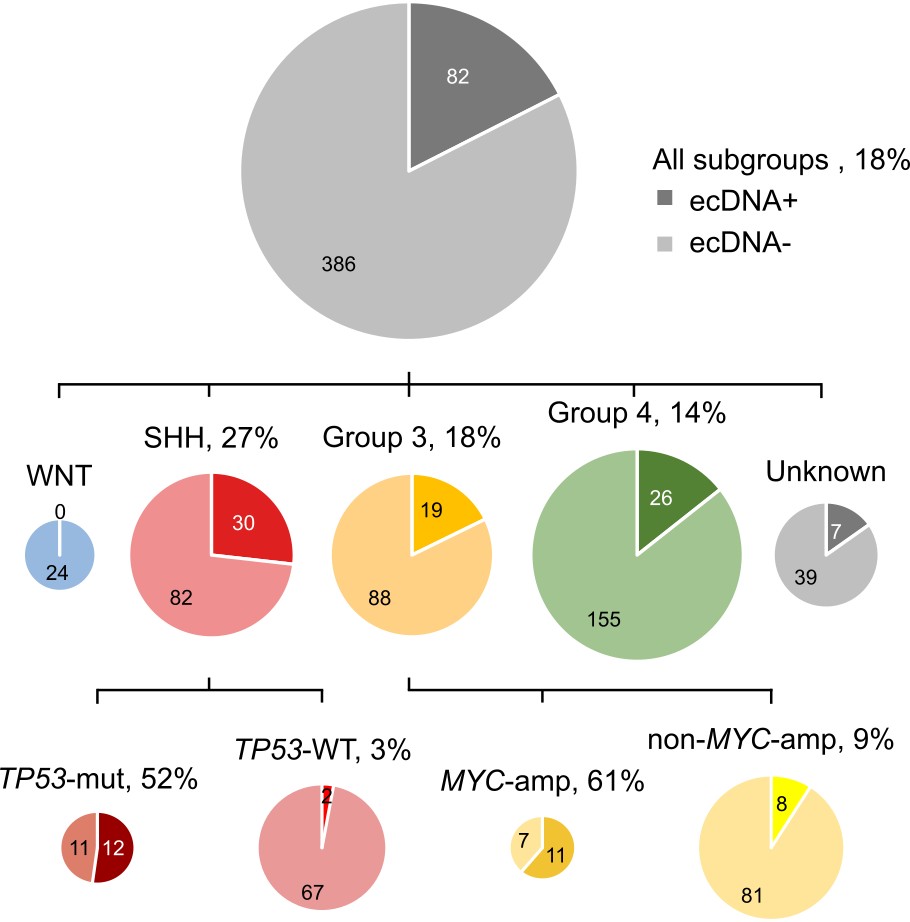
\includegraphics[]{figures/1-1.png}
    \caption[Presence of ecDNA by molecular subgroup across 468 MB patient tumors.]{\textbf{Presence of ecDNA by molecular subgroup across 468 MB patient tumors.} \textit{TP53}-mut/WT: \textit{TP53}-mutant/wild-type. \textit{MYC}-amp: \textit{MYC} copy number $\geq 5$ estimated from \gls{wgs}.}  
    \label{fig:1a}
\end{figure}

\begin{figure}[!h]
    \centering
    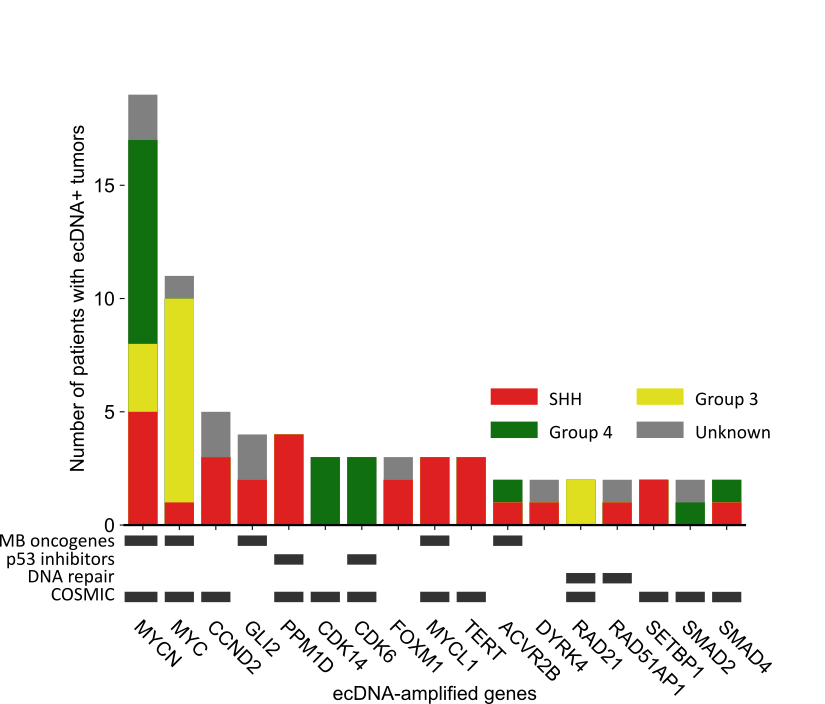
\includegraphics[]{figures/1-2.png}
    \caption[Recurrently amplified genes on ecDNA in MB.]{\textbf{Recurrently amplified genes on ecDNA in MB.} A subset of recurrently ($n \geq 2$) amplified genes on ecDNA in this patient cohort. p53 inhibitors: negative regulators of p53 pathway activity; COSMIC: genes listed as tier 1 or 2 of the COSMIC Cancer Gene Census \cite{cosmic}.}
    \label{fig:1b}
\end{figure}

\subsection{ecDNA predicts poor prognosis in medulloblastoma.}
To evaluate ecDNA as a potential prognostic marker in MB, we performed survival analyses across patients for whom clinical metadata were available. Patients with \gls{ecDNA+} tumors had significantly worse overall and progression-free 5-year survival (OS, PFS) compared to patients with ecDNA-negative tumors (ecDNA-) (log-rank test, $p < 0.005$; Fig. \ref{fig:km}). Stratified by molecular subgroup, ecDNA+ patients had worse overall survival in the SHH, Group 3 and Group 4 MB subgroups ($p<0.05$ for all subgroups; Fig. \ref{fig:km-subgroup}). Survival of WNT subgroup patients was not analyzed because no WNT tumors in our patient cohort were ecDNA+. To determine whether ecDNA+ patients had worse outcomes than patients with tumors harboring other types of focal somatic copy number amplification (fSCNA), we stratified patients by the topology of the amplification(s) present in the tumor genomes, using previously published methods \cite{Kim_2020}. As expected, ecDNA+ patients had the poorest clinical outcomes, significantly worse compared to patients without fSCNAs or with linear amplifications ($p<0.005$, Fig. \ref{fig:km-cna}). 

\begin{figure}[!h]
    \centering
    \begin{subfigure}{0.49\textwidth}
        \centering
        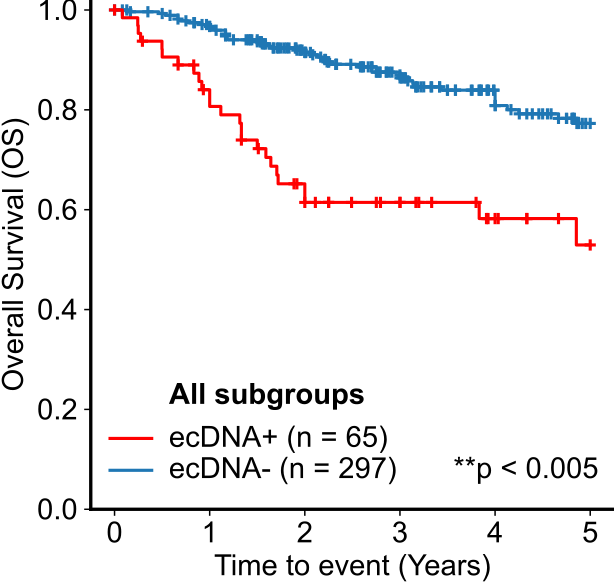
\includegraphics{p-KM-OS}
        \caption{}
        \label{subfig:os}
    \end{subfigure}
    \begin{subfigure}{0.49\textwidth}
        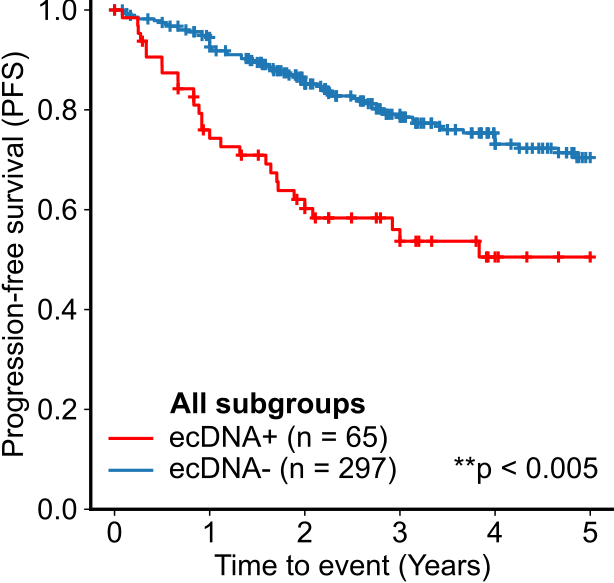
\includegraphics{p-KM-PFS}
        \caption{}
        \label{subfig:pfs}
    \end{subfigure}
    \caption[Survival of ecDNA+ and ecDNA- MB patients.]{\textbf{Survival of ecDNA+ and ecDNA- MB patients.} (\textbf{a}) 5-year overall survival and (\textbf{b}) progression-free survival of ecDNA+ and ecDNA- MB patients.}
    \label{fig:km}
\end{figure}

\begin{figure}[!h]
    \centering
    \begin{subfigure}{0.32\textwidth}
        \centering
        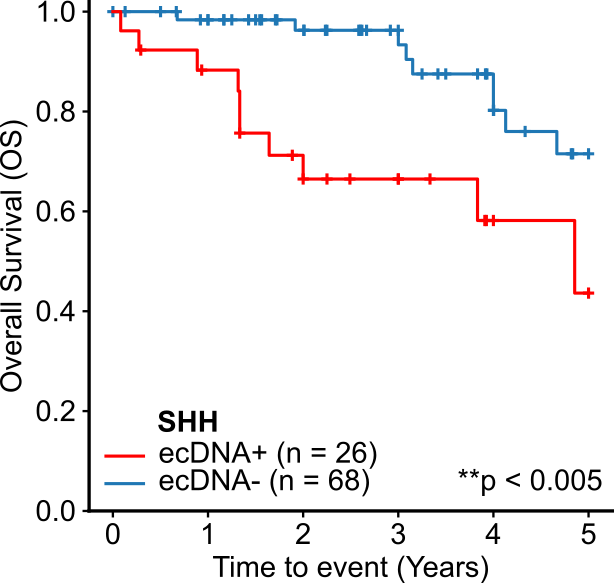
\includegraphics{p-KM-OS-SHH}
        \caption{}
        \label{subfig:os-shh}
    \end{subfigure}
    \begin{subfigure}{0.32\textwidth}
        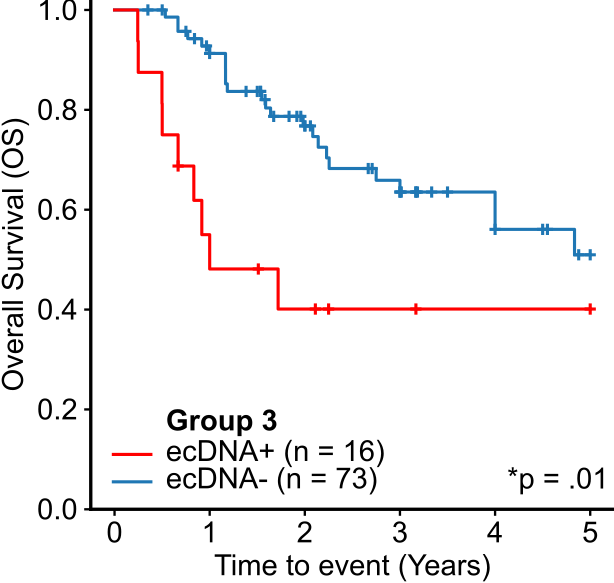
\includegraphics{p-KM-OS-G3}
        \caption{}
        \label{subfig:os-g3}
    \end{subfigure}
    \begin{subfigure}{0.32\textwidth}
        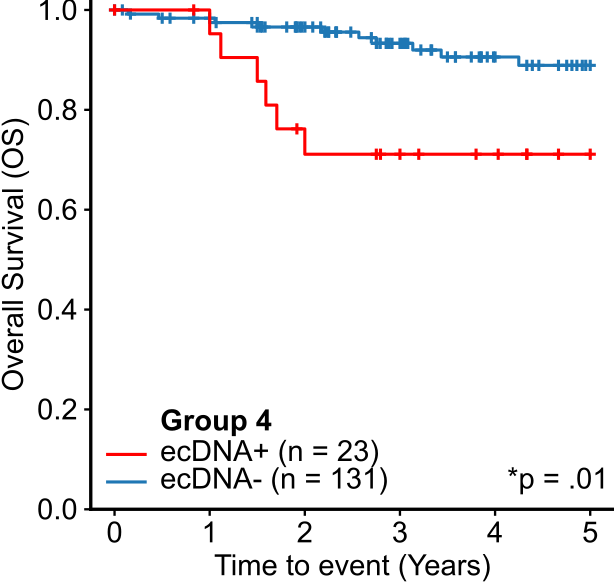
\includegraphics{p-KM-OS-G4}
        \caption{}
        \label{subfig:os-g4}
    \end{subfigure}
        \begin{subfigure}{0.32\textwidth}
        \centering
        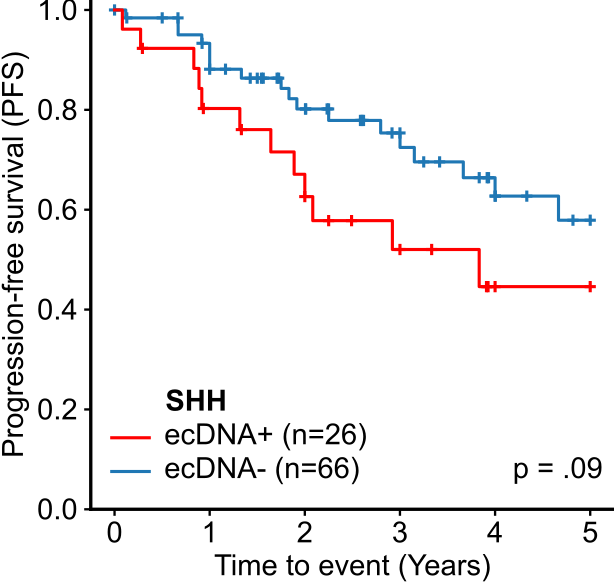
\includegraphics{p-KM-PFS-SHH}
        \caption{}
        \label{subfig:pfs-shh}
    \end{subfigure}
    \begin{subfigure}{0.32\textwidth}
        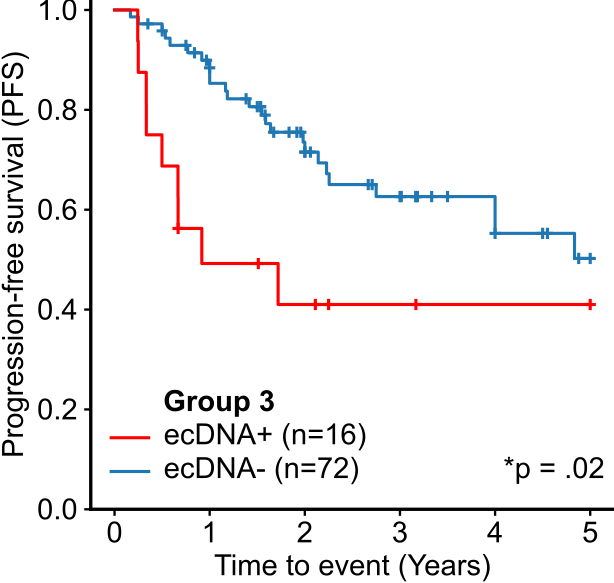
\includegraphics{p-KM-PFS-G3}
        \caption{}
        \label{subfig:pfs-g3}
    \end{subfigure}
    \begin{subfigure}{0.32\textwidth}
        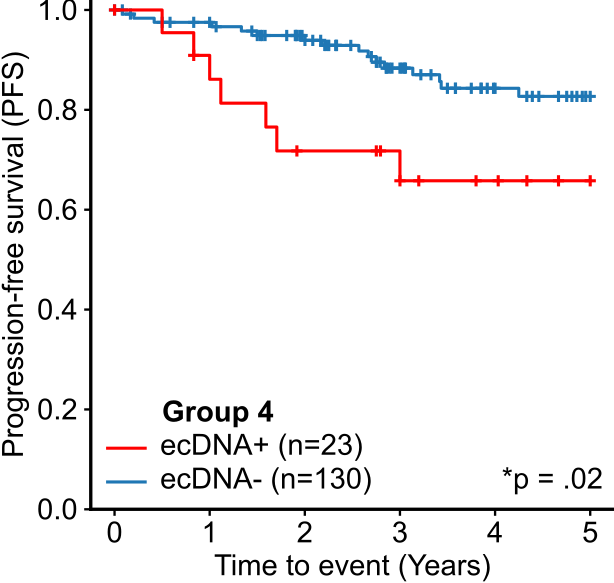
\includegraphics{p-KM-PFS-G4}
        \caption{}
        \label{subfig:pfs-g4}
    \end{subfigure}
    \caption[Survival of ecDNA+ and ecDNA- MB patients, stratified by molecular subgroup.]{\textbf{Survival of ecDNA+ and ecDNA- MB patients, stratified by molecular subgroup.} Survival curves indicating (\textbf{a-c}) 5-year overall survival and (\textbf{d-f}) progression-free survival of ecDNA+ and ecDNA- MB patients. \textbf{a-b}: SHH. \textbf{c-d}: Group 3. \textbf{e-f}: Group 4. WNT subgroup was not analyzed because ecDNA was not detected in WNT MB tumors.}
    \label{fig:km-subgroup}
\end{figure}

\begin{figure}[!h]
    \centering
    \begin{subfigure}{0.49\textwidth}
        \centering
        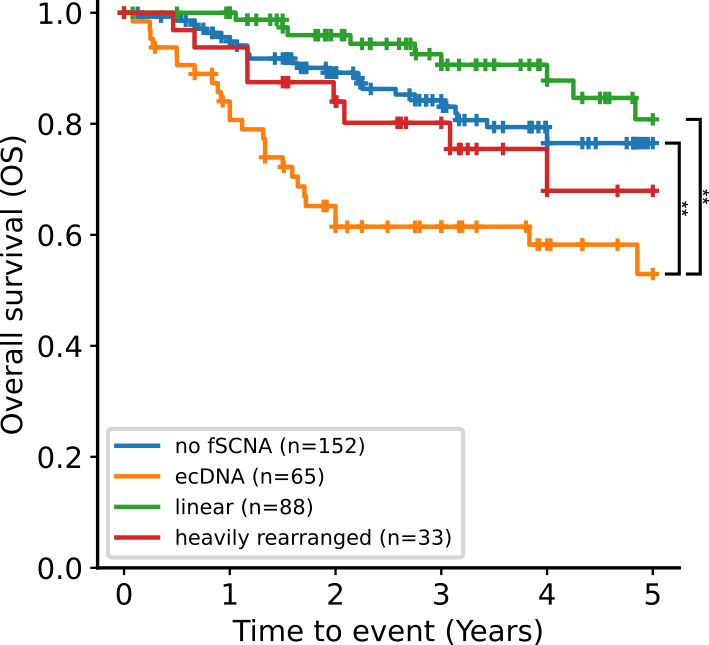
\includegraphics{p-KM-OS-subtypes}
        \caption{}
        \label{subfig:}
    \end{subfigure}
    \begin{subfigure}{0.49\textwidth}
        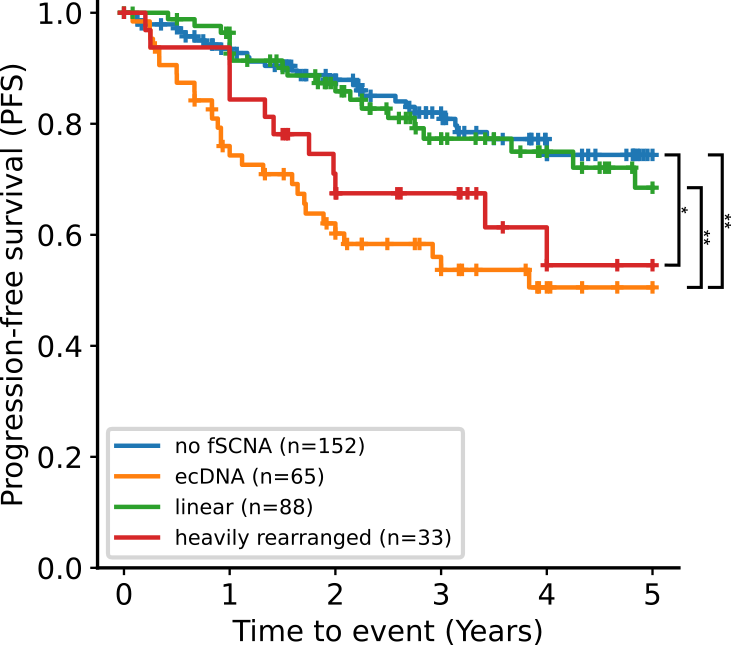
\includegraphics{p-KM-PFS-subtypes}
        \caption{}
        \label{subfig:}
    \end{subfigure}
    \caption[Survival of ecDNA+ and ecDNA- MB patients, stratified by focal somatic amplification(s) present.]{\textbf{Survival of ecDNA+ and ecDNA- MB patients, stratified by focal somatic amplification(s) present} in the tumor as classified by AmpliconClassifier \cite{Kim_2020}. ecDNA: tumor harbors a circular extrachromosomal amplification. Heavily rearranged: Tumor harbors an amplification classified as complex non-cyclic, but no cyclic ecDNA or BFB amplifications. Linear: Tumor harbors a linear amplification, but no highly-rearranged, BFB, or ecDNA amplifications. no fSCNA: no focal somatic copy number amplification detected.}
    \label{fig:km-cna}
\end{figure}

To further estimate the prognostic value of ecDNA, we conducted Cox proportional hazards models controlling for sex, age, and molecular subgroup. Patients with ecDNA+ tumors had greater estimated risk for progression (hazard ratio 2.36, $p < 0.005$) and mortality ($HR = 2.99$, $p < 0.005$) compared to patients with ecDNA- tumors (Fig. \ref{fig:cph-ssa}, Supplementary Table 2 of \cite{Chapman}). 

\begin{figure}[!h]
    \centering
    \begin{subfigure}{0.49\textwidth}
        \centering
        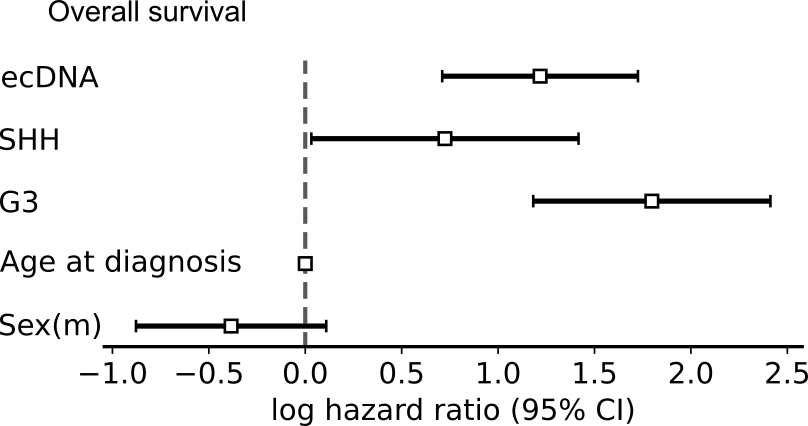
\includegraphics{p-CPH-OS-ssa}
        \caption{}
        \label{fig:cph-os-ssa}
    \end{subfigure}
    \begin{subfigure}{0.49\textwidth}
        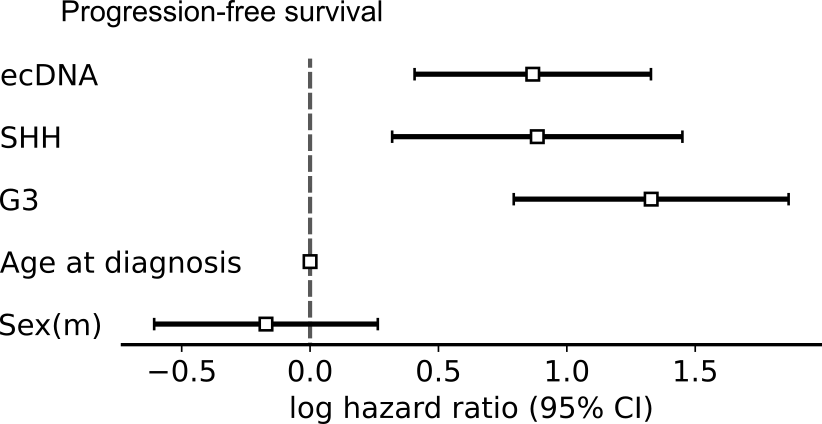
\includegraphics{p-CPH-PFS-ssa}
        \caption{}
        \label{fig:cph-pfs-ssa}
    \end{subfigure}
    \caption[Survival regressions on \gls{ecDNA}, MB subgroup, age and sex.]{\textbf{Survival regressions on \gls{ecDNA}, MB subgroup, age and sex.} Log hazard ratios for ecDNA status, MB subgroup, age and sex estimated by Cox proportional hazards regression on (\textbf{a}) overall survival and (\textbf{b}) progression-free survival. Model was fitted using \gls{mle}. Bars indicate 95\% confidence intervals. Estimated hazard ratios for ecDNA are $HR_{OS} = 2.99$, $p < 0.005$ and $HR_{PFS} = 2.36$, $p < 0.005$. }
    \label{fig:cph-ssa}
\end{figure}

\subsection{\textit{TP53} alterations are associated with ecDNA in SHH MB tumors.}
The tumor suppressor protein p53 (\textit{TP53}) is involved in DNA damage sensing, cell cycle arrest and apoptosis, and is frequently affected by somatic mutations and pathogenic germline variants in SHH MB \cite{Ramaswamy_2016, li-fraumeni_1988, waszak_2018}. Moreover, SHH-subgroup MBs with inactivating \textit{TP53} mutations are known to be associated with chromothripsis \cite{Rausch_2012}, a process of catastrophic shattering of a chromosome that has been shown to precede ecDNA formation in cell line models \cite{shoshani_2020, umbreit_2020}. To test whether \textit{TP53} mutations were associated with the presence of ecDNA in MB, we accessed the somatic and germline \textit{TP53} mutation status available for 92 SHH MBs. We found significant enrichment of \textit{TP53} alterations in ecDNA+ SHH MB tumors (12 of 23, 52\%) compared to ecDNA- SHH MB tumors (2 of 69, 3\%; $p=1.3e-7$, Fisher exact test; Table \ref{tab:shh-tp53}). We did not find a significant association between \textit{TP53} alterations and ecDNA either in the other MB subgroups or across the entire MB cohort, suggesting that in MB, a possible functional relationship between \textit{TP53} alterations and ecDNA is restricted to the SHH subgroup. 

%%%% TABLE 1 %%%%
\begin{table}[!ht]
\caption[\textit{TP53} mutation is associated with ecDNA in SHH subgroup MBs.]{\textbf{\textit{TP53} mutation is associated with ecDNA in SHH subgroup MBs.} We acquired somatic and germline mutation status of 92 SHH MBs from our patient cohort. Nearly every \textit{TP53}-mutant patient tumor contained ecDNA (12/14). The two without ecDNA showed evidence of breakage-fusion-bridge (BFB) amplification, a hypothesized precursor to ecDNA formation.}
\begin{center}
\begin{tabular}{ p{1in} p{1in} p{1in} }
\hline
 & \gls{ecDNA+} & ecDNA- \\
\hline
\textit{TP53}\textsubscript{mut} & 12 & 2 \\
\textit{TP53}\textsubscript{WT} & 11 & 67 \\
\hline
\end{tabular}
\end{center}
\label{tab:shh-tp53}
\end{table}

\par We hypothesized that the established effect of p53 mutation on SHH MB patient survival \cite{zhukova_2013} may be mediated, at least partially, by ecDNA (Fig. \ref{fig:aft}). To test this, we conducted mediation analyses using the Baron Kenny approach \cite{baron-kenny_1986}. Briefly, variable $M$ (ie, ecDNA status) is considered a mediator of the effect of independent variable $X$ (ie, p53 mutation) on outcome $Y$ (ie, patient survival) if (1) $X$ significantly predicts $Y$; (2) $X$ significantly predicts $M$; and (3) in a multiple regression of $Y$ on $X$ and $M$, $M$ significantly predicts $Y$ and the effect of $X$ on $Y$ is reduced relative to (1) (Fig. \ref{subfig:aft-model}) \cite{jung_2012}. To test (1), we fitted a log-normal \gls{aft} regression of \gls{pfs} parameterized on age, sex, molecular subgroup and p53 mutation status, using \gls{mle}. Without information on ecDNA, this model estimates that p53 mutation significantly reduces survival time by 77\% ($\mu = -1.46$, $p < 0.005$, Wald test; Fig. \ref{subfig:aft-p53}). For (2), we have already shown that p53 mutation strongly predicts the presence of ecDNA given molecular subgroup. To test (3), we refitted our AFT model parameterized on age, sex, molecular subgroup, p53 mutation, and ecDNA status. This model estimates that ecDNA significantly reduces survival time by 56\% ($\mu = -0.81$, $p < 0.005$; Fig. \ref{subfig:aft-p53-ecdna}). The same model estimates an insignificant reduction in survival time for p53 mutation, with a coefficient of lesser magnitude than that of (1) ($\mu = -0.94$, $p = 0.06$). We therefore concluded that the known prognostic effect of p53 mutation on survival may be partially  explained by an effect of ecDNA on prognosis and by the frequent co-occurrence of ecDNA in p53-mutant tumors.

\begin{figure}[!h]
    \centering
    \begin{subfigure}{\textwidth}
        \centering
        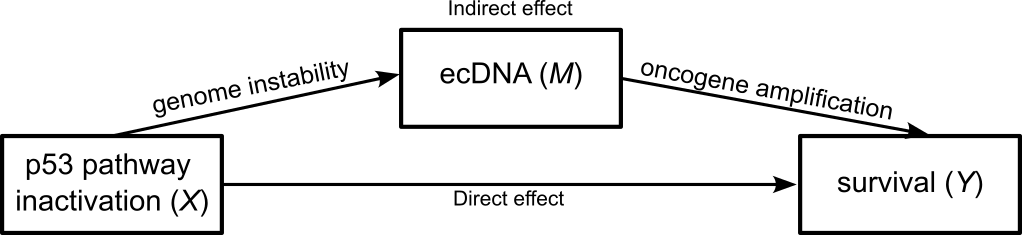
\includegraphics{1-4-1-mediation}
        \caption{}
        \label{subfig:aft-model}
    \end{subfigure}
    \centerline{%
    \begin{subfigure}{0.55\textwidth}
        \centering
        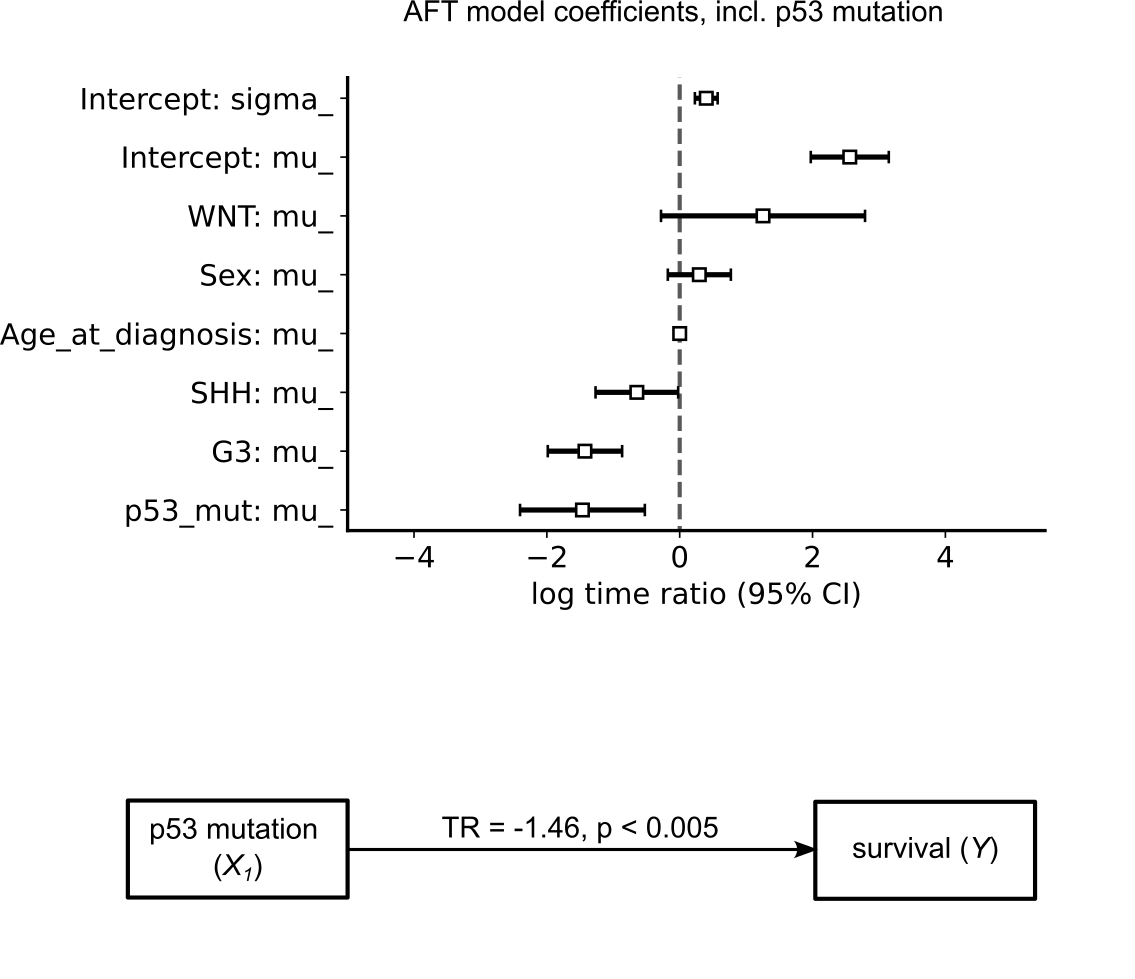
\includegraphics{p-AFT-PFS-p53}
        \caption{}
        \label{subfig:aft-p53}
    \end{subfigure}
    \begin{subfigure}{0.55\textwidth}
        \centering
        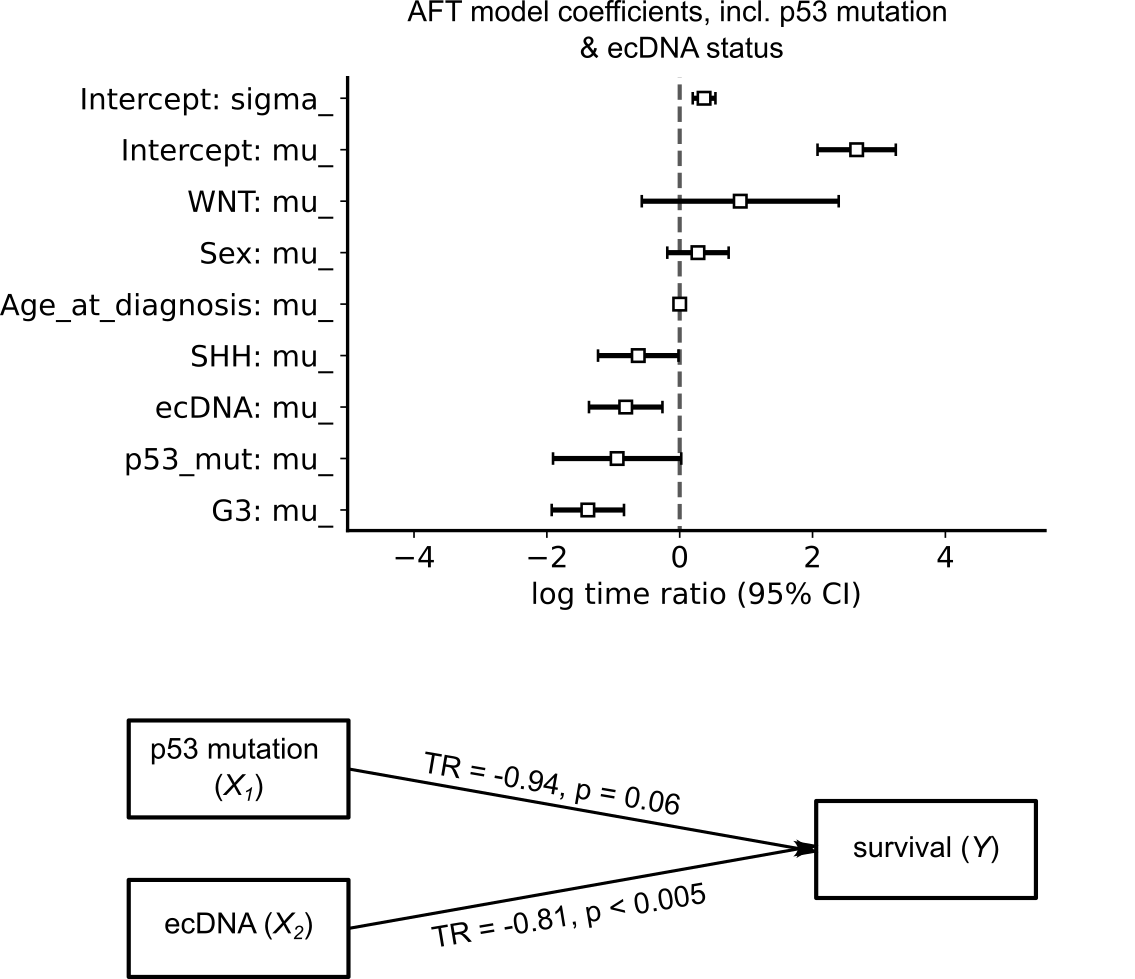
\includegraphics{p-AFT-PFS-p53-ecDNA}
        \caption{}
        \label{subfig:aft-p53-ecdna}
    \end{subfigure}%
    }
    \caption[Classical mediation analysis of associations between p53 mutation, \gls{ecDNA}, and patient outcomes.]{\textbf{Mediation analysis of p53 mutation, ecDNA, and progression-free survival.} (\textbf{a}) Model diagram of the proposed mediation relationship. p53 inactivation may predispose a tumor to form ecDNA, which then affects survival; p53 may also have ecDNA-independent effects on survival, eg. by formation of other structural variants. (\textbf{b}) Top: estimated time ratios for effects of age, sex, molecular subgroup and p53 mutation on \gls{pfs}. Bottom: effect size and p-value for p53 mutation are illustrated in the diagram below. (\textbf{c}) Top: estimated time ratios for effects of age, sex, molecular subgroup, p53 mutation, and ecDNA on \gls{pfs}. Bottom: effect size and p-values for p53 mutation and ecDNA are illustrated in the diagram below. The effect size of p53 on survival is decreased when controlling for ecDNA as a covariate, suggesting that ecDNA partially mediates the effect of p53 on survival.}
    \label{fig:aft}
\end{figure}

\par To evaluate whether there is a \textit{TP53}-independent effect of ecDNA on survival, we performed Cox regression including \textit{TP53} alteration as a covariate and controlling for collinearity. The effect of ecDNA on survival remains significant but diminished when we include p53 alteration as a covariate in our Cox models ($HR_{PFS} = 1.87, p = 0.01$; $HR_{OS} = 2.32, p < 0.005$; Fig. \ref{fig:cph-ssap}), indicating that there is an effect of ecDNA on survival that cannot be explained by p53 mutation alone. Such an effect may be explainable by a p53-independent mechanism of ecDNA formation, or by inactivation of the p53 pathway by other means such as \textit{CDKN2A} deletion or \textit{PPM1D}, \textit{CDK6}, \textit{MDM4} or \textit{MDM2} amplification \cite{mclendon_2008}. Although causality cannot be inferred from these data alone, our survival analyses identify \textit{TP53} alteration and ecDNA as clinically relevant biomarkers for a subset of highly aggressive SHH MB tumors. 

\begin{figure}[!h]
    \centering
    \centerline{%
    \begin{subfigure}{0.55\textwidth}
        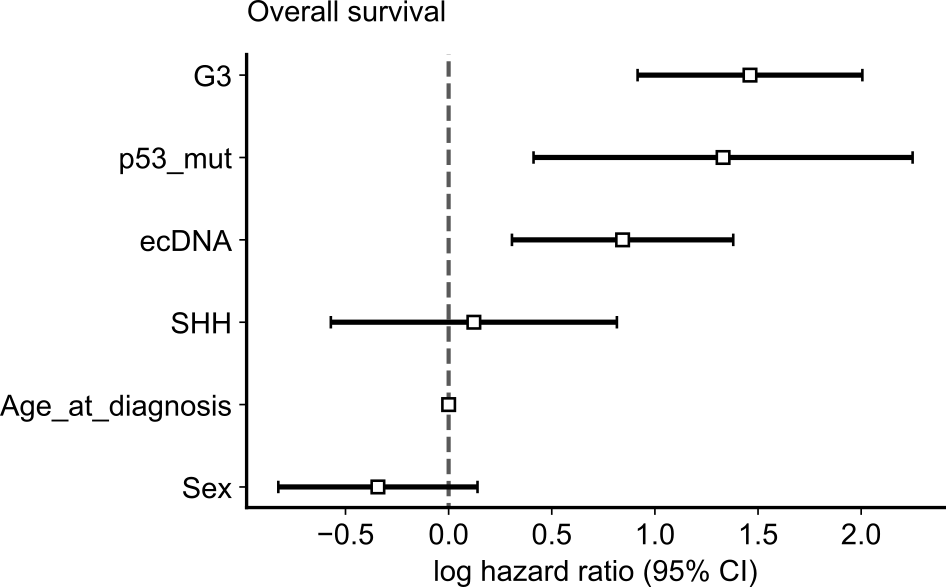
\includegraphics[right]{p-CPH-OS-ssap}
        \caption{}
        \label{subfig:cph-os-ssap}
    \end{subfigure}
    \begin{subfigure}{0.55\textwidth}
        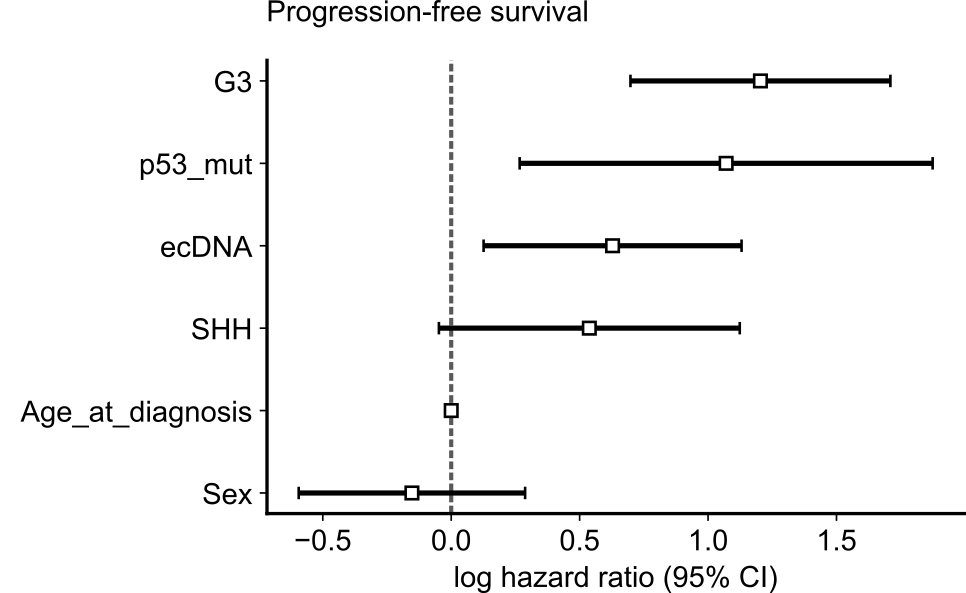
\includegraphics[left]{p-CPH-PFS-ssap}
        \caption{}
        \label{subfig:cph-pfs-ssap}
    \end{subfigure}%
    }
    \caption[Survival regressions on \gls{ecDNA} status, MB subgroup, age, sex, and p53 mutation.]{\textbf{Survival regressions on \gls{ecDNA} status, MB subgroup, age, sex, and p53 mutation.} Log hazard ratios for ecDNA status, MB subgroup, age, sex, and p53 mutation estimated by Cox proportional hazards regression on (\textbf{a}) overall survival and (\textbf{b}) progression-free survival. Model was fitted using ridge regression to control for collinearity. Bars indicate 95\% confidence intervals. Estimated hazard ratios for ecDNA are $HR_{OS} = 2.32, p < 0.005$; $HR_{PFS} = 1.87, p = 0.01$. }
    \label{fig:cph-ssap}
\end{figure}

\section{Discussion}

\par As in other cancers \cite{Turner_2017,Kim_2020,luebeck_2022}, ecDNA frequently amplifies known oncogenic MB driver genes. Our results identify ecDNA as a frequent feature of \textit{MYC}-amplified Group 3 and p53-mutant SHH tumors, which share exceptionally poor prognoses \cite{Ryan_2012,Rausch_2012} but few other recurrent driver mutations. Recent longitudinal analysis of Barrett’s esophagus suggests that \textit{TP53} alteration is an early event in ecDNA-driven malignant transformation \cite{luebeck_2022}. However, the absence of detectable ecDNA in \textit{TP53}-mutant WNT subgroup tumors, and the frequent occurrence of ecDNA in Group 3 tumors with wild type \textit{TP53}, suggest that the mechanisms for the generation and selection of tumor cells with ecDNA are MB subgroup-specific and thus may be modulated by the different cellular contexts of MB progenitor cells.

\par A long-standing problem in the clinical management of medulloblastoma tumors has been the paucity of effective targeted molecular treatments for MB, especially in relapsed cases. For example, the SMO inhibitor vismodegib, one of few targeted drugs approved for SHH medulloblastoma, is ineffective against \textit{TP53}-mutant, \textit{MYCN}-amplified or \textit{GLI2}-amplified tumors \cite{robinson_2015}, each a recurrent feature of ecDNA+ MB in our patient cohort. Through a retrospective analysis of one of the largest cohorts of \gls{wgs} and clinical outcome data from MB patients assembled to date, we demonstrate that the occurrence of ecDNA significantly associates with poor outcome across the entire cohort and within individual MB subgroups. Our survival analysis estimates that relative to ecDNA- patients, ecDNA+ MB patients are more than twice as likely to relapse and three times as likely to die during the follow-up interval. The identification of MB patients with ecDNA is therefore crucial to pave the way for precision medicine approaches targeting ecDNA-specific properties.

\section{Methods}
\label{chap1:methods}
\subsection{Statistical methods}
Statistical test, test statistic and p-values are indicated where appropriate in the main text. Categorical associations were established using the chi-squared test of independence if $N>5$ for all categories, and Fisher exact test otherwise. For both tests, the python package scipy.stats v1.5.3 implementation was used \cite{scipy}. Multiple hypothesis corrections were performed using the Benjamini-Hochberg correction \cite{bh} implemented in statsmodels v0.12.0 \cite{statsmodels}. All statistical tests described herein were two-sided unless otherwise specified.

\subsection{Medulloblastoma WGS}
Paired-end whole genome sequencing (WGS) data were acquired for each of the sources described below. In total the WGS cohort comprised 468 patients, 4 cell lines and 26 PDX models. Unless otherwise specified, WGS was acquired for 1 tumor biosample per patient.

\subsubsection{CBTN -- Children's Brain Tumor Network (114 biosamples from 101 patients)} WGS of medulloblastoma tumor biopsies were identified using the Gabriella Miller KidsFirst Data Resource center portal (\url{https://portal.kidsfirstdrc.org/}) on 29 May 2020. Patients were originally sequenced as part of the Pediatric Brain Tumor Atlas (PBTA) (\url{https://cbtn.org/pediatric-brain-tumor-atlas}). WGS data were preprocessed and aligned using the KidsFirst harmonized WGS pipeline (hg38) and subsequently analyzed using Cavatica (\url{https://cavatica.sbgenomics.com/}), on the cloud genomic analysis platform for KidsFirst genomic data. Docker containers containing fingerprint and AmpliconArchitect software were installed on the Cavatica cloud genomics platform (see Methods: ``EcDNA detection and classification").

\subsubsection{St Jude (79 patients)} WGS of MB biopsies were identified using the St Jude Cloud Data Portal (\url{https://platform.stjude.cloud/data/}) on 11 February 2020. WGS was preprocessed and aligned by bwa-mem to hg38 as described in McLeod et al31. Docker containers of fingerprint and AmpliconArchitect software were installed on the DNANexus cloud genomics platform (see Methods: ``EcDNA detection and classification").
\subsubsection{ICGC - International Cancer Genome Consortium (237 patients)} WGS of MB tumor biopsies was identified using the ICGC Data Portal (\url{https://dcc.icgc.org/}) on 12 May 2020 and downloaded from the Collaboratory cloud genomics platform using the ICGC Score download client. These tumor genomes were previously sequenced, aligned and deposited with ICGC in other publications (GRCh37)\cite{Northcott_2017,pcawg}.

\subsubsection{Archer \textit{et al.} (43 patients)} All WGS data for these 43 patients were previously published elsewhere\cite{Northcott_2017}. Sequencing data were aligned to human genome reference GRCh37 processed according to the best practice pipelines at the Cancer Genome Analysis group at the Broad Institute\cite{archer_2017}.

\subsubsection{Rady Children's Hospital (8 patients)} Tumor biopsies were collected and consented for research as part of the Rady Molecular Tumor Board (MTB). Paired end reads were acquired from Rady's Children hospital. Sequencing depth for all samples were at least 30x. Raw fastq reads were aligned to UCSC hg38 coordinates using BWA v0.7.17-r1188 \cite{bwa}.  Reads were sorted by samtools v0.1.19 \cite{samtools}, marked for duplicates with Picard Tools v2.12.3, and recalibrated with GATK v3.8-1-0 \cite{mckenna_2010,depristo_2011,vanderauwera_2013}.

\subsubsection{Cell lines and PDX models (4 cell lines, 26 PDXs)} Low-coverage WGS for 19 PDX models and 9 corresponding origin human tumors were obtained from a previous publication \cite{rusert_2020}. An additional 6 PDX biosamples (RCMB25, RCMB32, RCMB56, RCMB57, RCMB58 and RCMB69) were contributed by Wechsler-Reya lab using similar methods to establish PDX lines. Cell lines (D283, D341, D425 and D458) were contributed by Bagchi (SBP), Taylor (U. Toronto) and Wechsler-Reya (SBP) labs. WGS was performed at the UCSD IGM Genomics and Sequencing Core (hg38) for all samples except D283, for which no WGS was obtained. Preprocessing and alignment was performed using the same protocol as the RCH patient biopsies above.
\subsection{ecDNA detection and classification from bulk WGS}
To detect ecDNA, all samples in the WGS cohort were analyzed using AmpliconArchitect \cite{AA} v1.2 and AmpliconClassifier \cite{Kim_2020} v0.4.4. Briefly, the AmpliconArchitect algorithm was performed as follows. Copy number segmentation and estimation were performed using CNVkit v0.9.6 \cite{cnvkit}. Segments with copy number $\geq 4$ were extracted using AmpliconSuite-pipeline (April 2020 update) as ``seed" regions. For each seed, AmpliconArchitect searches the region and nearby loci for discordant read pairs indicative of genomic structural rearrangement. Genomic segments are defined based on boundaries formed by genomic breakpoint locations (identified by discordant reads) and by modulations in genomic copy number. A breakpoint graph of the amplicon region is constructed using the CN-aware segments and the genomic breakpoints, and cyclic paths are extracted from the graph.  Amplicons are classified as ecDNA, breakage-fusion-bridge, complex, linear, or no focal amplification by the heuristic-based companion script, AmpliconClassifier. Biosamples with one or more classifications of ``ecDNA" were considered potentially ecDNA+, and all others were considered ecDNA- (Supplementary Table 1c from \cite{Chapman}). We manually reviewed all potential ecDNA+ assembly graphs and reclassified those with inconclusive ecDNA status, which we defined as any of the following:
\begin{itemize}
    \item Low-copy amplification ($<5$) AND no copy number change at discordant read breakpoints
    \item Cycles consisting of the repetitive region at chr5:820000 (GRCh37).
\end{itemize}
Code is available at:
\begin{itemize}
    \item AmpliconSuite-pipeline: \url{https://github.com/jluebeck/AmpliconReconstructor}
    \item AmpliconArchitect: {https://github.com/jluebeck/AmpliconArchitect} 
    \item AmpliconClassifier: \url{https://github.com/jluebeck/AmpliconClassifier} 
\end{itemize}
The ecDNA- status of the D283 cell line was not determined computationally by WGS, but by copy number analysis of DNA methylation, FISH (see Methods: ``FISH").
\subsection{Fingerprinting analysis}
To uniquely identify WGS from each patient, we counted reference and alternate allele frequencies at 1000 variable non-pathogenic SNP locations in the human genome according to the 1000 Genomes project \cite{1000_genomes}, and performed pairwise Pearson correlation between all WGS samples. Biospecimens originating from the same patient tumor (eg., primary/relapse or origin/PDX pairs) were readily distinguishable by high correlation across these sites ($r > 0.80$). We identified one case in our cohort in which 2 tumor biosamples had highly correlated fingerprints: MDT-AP-1217.bam and ICGC\_MB127.bam. We arbitrarily removed ICGC\_MB127 from the patient cohort. 
\subsection{Patient metadata, survival, and medulloblastoma subgroup annotation.}
Where available, patient samples and models were assigned metadata annotations including age, sex, survival, and MB subgroup based on previously published annotations of the same tumor or model \cite{archer_2017,Northcott_2017,waszak_2018,rusert_2020,ivanov_2016,robinson_2012,northcott_2012}. Sample metadata are also available in some cases from the respective cloud genomics data platform: \url{https://dcc.icgc.org/} (ICGC), \url{https://pedcbioportal.kidsfirstdrc.org/} and \url{https://portal.kidsfirstdrc.org/} (CBTN), and \url{https://pecan.stjude.cloud/} (St Jude). Where primary sources disagreed on a metadata value, that value was reassigned to NA. Patient tumors from the CBTN were assigned molecular subgroups based on consensus of 2 molecular classifiers using RSEM-normalized FPKM data: MM2S \cite{gendoo_2016} and the D3b medulloblastoma classifier at the Children's Hospital of Philadelphia (\url{https://github.com/d3b-center/medullo-classifier-package}). To determine molecular subgroup of PDX samples, we generated or obtained from a previous publication \cite{rusert_2020} DNA methylation profiles (Illumina 450k or EPIC) and classified samples by molecular subgroup according to the DKFZ brain tumor methylation classifier (\url{https://www.molecularneuropathology.org/mnp}) \cite{Northcott_2017}.
\subsection{\textit{TP53} mutation annotation}
\subsubsection{Somatic mutations} Somatic \textit{TP53} mutation information for the ICGC and CBTN cohorts was acquired from a previous publication \cite{waszak_2018} and from the ICGC and CBTN data portals (see Methods\: "Patient metadata, survival, and subgroup annotation". Somatic \textit{TP53} mutation information for the St. Jude cohort was extracted from the standard internal St. Jude variant calling pipeline \cite{stjude}. Somatic mutations were only considered which were protein-coding and missense, nonsense, insertion or deletion, or affected a splice site junction.

\subsubsection{Germline variants} Whole-genome sequencing (WGS) GVCF files were downloaded from the ICGC data portal (\url{https://dcc.icgc.org/}), the KidsFirst data portal (\url{https://portal.kidsfirstdrc.org/dashboard}) and DNAnexus for St. Jude Pediatric Cancer Genome Project (PCGP). xGVCF files were merged with GLnexus \cite{glnexus} and converted to PLINK format for analysis of ICGC, PCGP and KidsFirst genotypes. PCGP genotypes were converted to hg19 coordinates using liftover. Variants from \textit{TP53} genomic locus (hg19\:chr17\:7571739-759080) were extracted and annotated with REVEL \cite{revel_2016}, CADD \cite{cadd}, ClinVar (accessed June 2021) and Variant Effect Predictor (VEP) \cite{vep}. REVEL GRCh38 scores were downloaded from \url{https://sites.google.com/site/revelgenomics/} (date accessed: 03/05/2021). CADDv1.6 scores were downloaded from \url{https://cadd.gs.washington.edu/info} (date accessed: 03/23/2020). VEP scores were calculated with \url{http://grch37.ensembl.org/index.html} release 104 (date accessed: 04/27/21). Clinvar scores were obtained from \url{https://ftp.ncbi.nlm.nih.gov/pub/clinvar/vcf_GRCh37/} (Date accessed: 04/27/21). VEP variants considered pathogenic included "frameshift" and ``splice" variants. ClinVar annotations considered pathogenic included ``frameshift", ``stop", ``splice", and ``deletion", and whose clinical significance were ``pathogenic" or ``likely pathogenic". CADD ``pathogenic" variants had a CADD score of at least 10 (Phred score). REVEL ``pathogenic" variants had a REVEL score of at least 0.5. Only variants with minor allele frequency (MAF) less than 5\%, according to the gnomAD r2.1.1 database, were analyzed \cite{karczewski_2020}.

\subsection{Survival analyses}
\acrfull{km}, \acrfull{cph}, and \acrfull{aft} analyses were performed with Lifelines v0.26.5 \cite{lifelines}. For all analyses, the sample set was all patients annotated with the included covariates; no imputation was performed. 
\subsubsection{Kaplan-Meier} Sample sizes were $n = 362$ (65 ecDNA+; 297 ecDNA-). Differential survival was determined by log-rank test. For \acrshort{km} analyses by class of structural variant, samples were classified as previously described \cite{Kim_2020}. Our sample of patients with breakage-fusion-bridge (BFB) amplification but no ecDNA was too small to test ($n=2$).
\subsubsection{Cox Proportional Hazards on age, sex, molecular subgroup, \& ecDNA} Sample was $n = 352$ observations. Model was fitted by maximum likelihood estimation (MLE).
\subsubsection{Cox Proportional Hazards on age, sex, molecular subgroup, p53 mutation, \& ecDNA} Sample was $n = 322$ observations. Collinearity, \textit{i.e.} strong correlation between predictive variables in a regression model, can result in model instability and unreliable estimation of the collinear coefficients \cite{liu_2017}. To address collinearity between ecDNA and p53 status in our model, we performed ridge estimation of model coefficients \cite{verweij_1994, xue_2007}, determining the ridge penalty parameter $\lambda$ by grid search on 5-fold cross validation of model likelihood on the withheld set.
\subsubsection{Accelerated failure time models and mediation analysis} Mediation analysis was performed using the Baron-Kenny framework \cite{baron-kenny_1986}, following recent best practices \cite{lapointe_2018}. Because of the non-collapsibility of hazard ratios, the proportional hazards assumption and \acrshort{cph} model may not be suitable for mediation analysis in which we need to compare the coefficients with and without the mediator. Thus, we fitted we fitted parametric log-normal \acrshort{aft} regression models as a reasonable alternative to Cox regression. Percent change values reported herein were calculated as
$$\textsc{Percentage Change}=100(e^{\hat{\beta}_k}-1),$$
 where  $\hat{\beta}_k$ is the MLE regression coefficient for random variable $k$ \cite{demeritt_2022}. 

\section{Acknowledgments}

\ackfunding

\par Chapter 1, in full, is adapted from the following manuscript currently being prepared for publication: "Circular extrachromosomal DNA promotes inter- and intratumoral heterogeneity in high-risk medulloblastoma." Chapman, Owen; Luebeck, Jens; Sridhar, Sunita; Wong, Ivy T.L.; Dixit, Deobrat; Wang, Shanqing; Prasad, Gino; Rajkumar, Utkrisht; Pagadala, Meghana; Larson, Jon D.; He, Britney J.; Hung, King L.; Lange, Joshua T.; Dehkordi, Siavash R.; Chandran, Sahaana; Adam, Miriam; Morgan, Ling; Wani, Sameena; Tiwari, Ashutosh; Guccione, Caitlin; Lin, Yingxi; Dutta, Aditi; Lo, Yan Yuen; Juarez, Edwin; Robinson, James T.; Malicki, Denise M.; Coufal, Nicole G.; Levy, Michael; Hobbs, Charlotte; Scheuermann, Richard H.; Crawford, John R.; Pomeroy, Scott L.; Rich, Jeremy; Zhang, Xinlian; Chang, Howard Y.; Dixon, Jesse R.; Bagchi, Anindya; Deshpande, Aniruddha J.; Carter, Hannah; Fraenkel, Ernest; Mischel, Paul S.; Wechsler-Reya, Robert J.; Bafna, Vineet; Mesirov, Jill P.; Chavez, Lukas. The dissertation author was the primary investigator and author of the manuscript.

%%%%%%%%%%%%%%%%%%%%